% !TEX encoding = UTF-8
%Koma article
\documentclass[fontsize=12pt,paper=letter,twoside]{scrartcl}
\usepackage{float}
\usepackage{url}
\usepackage{listings}

%For Code Stylings
\usepackage{listings}
\usepackage{color}

\definecolor{mygreen}{rgb}{0,0.6,0}
\definecolor{mygray}{rgb}{0.5,0.5,0.5}
\definecolor{mymauve}{rgb}{0.58,0,0.82}

\lstset{ 
  backgroundcolor=\color{white},   % choose the background color; you must add \usepackage{color} or \usepackage{xcolor}; should come as last argument
  basicstyle=\tiny,        % the size of the fonts that are used for the code
  breakatwhitespace=false,         % sets if automatic breaks should only happen at whitespace
  breaklines=true,                 % sets automatic line breaking
  captionpos=b,                    % sets the caption-position to bottom
  commentstyle=\color{mygreen},    % comment style
  deletekeywords={...},            % if you want to delete keywords from the given language
  escapeinside={\%*}{*)},          % if you want to add LaTeX within your code
  extendedchars=true,              % lets you use non-ASCII characters; for 8-bits encodings only, does not work with UTF-8
  frame=single,	                   % adds a frame around the code
  keepspaces=true,                 % keeps spaces in text, useful for keeping indentation of code (possibly needs columns=flexible)
  keywordstyle=\color{blue},       % keyword style
  language=Octave,                 % the language of the code
  morekeywords={*,...},            % if you want to add more keywords to the set
  numbers=left,                    % where to put the line-numbers; possible values are (none, left, right)
  numbersep=5pt,                   % how far the line-numbers are from the code
  numberstyle=\tiny\color{mygray}, % the style that is used for the line-numbers
  rulecolor=\color{black},         % if not set, the frame-color may be changed on line-breaks within not-black text (e.g. comments (green here))
  showspaces=false,                % show spaces everywhere adding particular underscores; it overrides 'showstringspaces'
  showstringspaces=false,          % underline spaces within strings only
  showtabs=false,                  % show tabs within strings adding particular underscores
  stepnumber=2,                    % the step between two line-numbers. If it's 1, each line will be numbered
  stringstyle=\color{mymauve},     % string literal style
  tabsize=1,	                   % sets default tabsize to 2 spaces
  title=\lstname                   % show the filename of files included with \lstinputlisting; also try caption instead of title
}
%Standard Pre-amble
\usepackage[top=4cm,bottom=4cm,left=3cm,right=3cm,asymmetric]{geometry}
%\geometry{landscape}                % Activate for for rotated page geometry
%\usepackage[parfill]{parskip}    % Begin paragraphs with an empty line rather than an indent
\usepackage[table,xcdraw]{xcolor}
\usepackage{graphicx}

\usepackage{amsmath}
\usepackage{amssymb}
\usepackage{epstopdf}
\DeclareGraphicsRule{.tif}{png}{.png}{`convert #1 `dirname #1`/`basename #1 .tif`.png}
% Listings needs package courier
\usepackage{listings} % Needs 
\usepackage{courier}

\usepackage[framemethod=TikZ]{mdframed}
\usepackage{url}

\usepackage{sty/bsymb} %% Event-B symbols
\usepackage{sty/eventB} %% REQ and ENV
\usepackage{sty/calculation}

%Maths
\usepackage{amssymb,amsmath}
\def\Fl{\mathbb{F}}
\def\Rl{\mathbb{R}}
\def\Nl{\mathbb{N}}
\def\Bl{\mathbb{B}}
\def\St{\mathbb{S}}
\newcommand{\ovr}{\upharpoonright}
\newcommand{\var}[1]{\textit{#1}}
%Useful definitions
\newcommand{\mv}[1]{\textit{m\_#1}}
\newcommand{\cv}[1]{\textit{c\_#1}}
\newcommand{\degree}[1]{^{\circ}\mathrm{#1}}
%\newcommand{\comment}[1]{{\footnotesize \quad\texttt{--}\textrm{#1}}}
\newcommand{\im}[1]{i\texttt{-\!#1}}

\usepackage[headsepline]{scrpage2}
\pagestyle{scrheadings}
\ihead[]{\small EECS4312 Report1}
\ohead[]{\small \thepage}
\cfoot[]{}
\ofoot[]{}


%%%%PVS environment%%%%%%%%%%%%%%%%%%%
\lstnewenvironment{pvs}[1][]
    {\lstset{#1,captionpos=b,language=pvs,
    mathescape=true,
    basicstyle=\small\ttfamily,
    numbers=none,
    frame=single,
    % numberstyle=\tiny\color{gray},
    % backgroundcolor=\color{lightgray},
    firstnumber=auto
    }}
    {}
 %%%%%%%%%%%%%%%%%%%%%%%%%%%%%%%%
 
%%%%Verbatim environment%%%%%%%%%%%%%%%%%%%
\lstnewenvironment{code}[1][]
    {\lstset{#1,captionpos=b,
    mathescape=true,
    basicstyle=\small\ttfamily,
    numbers=none,
    frame=single,
    % numberstyle=\tiny\color{gray},
    % backgroundcolor=\color{lightgray},
    firstnumber=auto
    }}
    {}

% \newenvironment{boxed}[1]
%    {\begin{center}
%    #1\\[1ex]
%    \begin{tabular}{|p{0.9\textwidth}|}
%    \hline\\
%    }
%    { 
%    \\\\\hline
%    \end{tabular} 
%    \end{center}
%    }
 %%%%%%%%%%%%%%%%%%%%%%%%%%%%%%%%
 
 %Text in a box
\newenvironment{textbox}
    {\begin{center}
    \begin{tabular}{|p{0.9\textwidth}|}
    \hline\\
    }
    { 
    \\\\\hline
    \end{tabular} 
    \end{center}
    }

\usepackage{hyperref}

%Highlight \hl{}
\usepackage{soul}

\usepackage{enumitem}
\newlist{mylist}{itemize}{1}
\setlist[mylist]{label=\textbullet,leftmargin=1cm,nosep}

\usepackage{multirow}

% Reduce space between figure and caption
%\usepackage{caption}
%\captionsetup[table]{font=small,skip=0pt}     %% Adjust here
%or equivalently 
\usepackage[font=small,skip=4pt]{caption}
%Useful definitions
%\newcommand{\mv}[1]{\textit{m\_#1}}
%\newcommand{\cv}[1]{\textit{c\_#1}}
%\newcommand{\degree}[1]{^{\circ}\mathrm{#1}}
%\newcommand{\comment}[1]{{\footnotesize \quad\texttt{--}\textrm{#1}}}

% Set the header
\ihead[]{\small EECS4090 Project}


%%%%%%%%%%%%Enter your names here%%%%%%%%
\author{\textbf{Edward Vaisman}
\and \textbf{Sadman Sakib Hasan}
}
%%%%%%%%%%%%%%%%%%%%%%%%%%%%%%%%

\date{\today} % Display a given date or no date

\begin{document}
\title{Grad Apps 2.0 Design Documentation}
\maketitle

\newpage

\section*{Revisions}

%%%%%%%%%%%%Table of revisions%%%%%%%%
\begin{tabular}{|l|l|p{3in}|}
\hline
Date & Revision & Description \\ 
\hline
22 November, 2017
& 1.0
& Initial Document Draft \\
\hline
4 December, 2017
& 1.1
& Included UML Class Diagram and Rationale \\
\hline
12 December, 2017
& 1.2
& Updated the Class diagram (Model section Role separation), Added Entity-Model Diagram, Added Data descriptions \\
\hline
14 December, 2017
& 1.3
& Updated Class diagram to match the new model, Updated Entity-Model Diagram, Edited Data descriptions \\
\hline
16 December, 2017
& 1.4
& Added Interface Design and Traceability Matrix \\
\hline
17 December, 2017
& 1.5
& Added Sequence Diagrams for the Component Design \\
\hline
19 January, 2018
& 1.6
& Updated Data Dictionary and Model Diagram \\
\hline
\hl{28 April, 2018}
& 1.7
& Updated Data Dictionary, ER Diagram, and added File Structure. Removed Requirements Matrix \& Appendices\\
\hline
\end{tabular}
%%%%%%%%%%%%%%%%%%%%%%%%%%%%%%%%

\newpage

%%%%%%%%%%%%%%%%%%%%%%%%%%%%%%%
\tableofcontents
\listoffigures
\newpage


%%%%Rest of your document goes here%%%%%%%%%%%%%%%%%%%

\clearpage
\section{Introduction}

\subsection{Purpose}

This software design document is intended to provide information regarding the system and architecture on the design of the new graduate application system for the EECS graduate program.

\subsection{Scope}

Gradapps v2.0, a graduate application system, is intended to assist the EECS graduate program better locate and maintain potential graduate student applications from the moment it is submitted until the moment a decision is made. It is intended to replace the current system in use for the EECS graduate program. It will be accessible for use as an online portal on the web.

\smallskip
\noindent Gradapps v2.0 promises the following:
\begin{itemize}
\item \emph{Administrators} will be able to manage \emph{Committee Members}, assign applications to \emph{Committee Members} to review, edit/manage student applications, grant/revoke privileges from faculty members and add/remove members from the system.
\item \emph{Committee Members} will be able to view and manage a list of student applications assigned to them and be able to save applications as a draft for future edits.
\item \emph{Professors} will be able to search for applications and indicate their interest in a student to other professors and for personal use indicate whether or not an application has been reviewed.
\item All roles will be able to apply advanced filtering methods relative to their given roles to help search for applications.
\end{itemize}

\newpage
\subsection{Overview}

This document is divided into 9 sections,

\begin{itemize}
\item Introduction
\item System Overview
\item System Architecture
\item Data Design
\item Component Design
\item Human Interface Design
\end{itemize}

%%%%%%%%%%%%%%%%%%%%%%%%%%%%%%%%%%%%%%%%%%%

\newpage
\section{System Overview}

Having a postgraduate degree on one's resume is always appealing to their future employer, let it be working in the industry or continuing studies to achieve a doctoral status. When applying for a postgraduate program, applicants spend a lot of their time gathering different levels of information (transcripts, letter of recommendation, resume etc.) required for admission. Once an application has been submitted, the graduate program analyses the information to find the best candidate for each program.

\smallskip
Analysing that level of dense information can be challenging at times and to avoid loss of any information, it is best practice to automate this process as much as possible. In order to achieve that goal, a \emph{concise} and \emph{simple} Business System is required that will reduce the manual work.

\smallskip
The graduate program in Electrical Engineering and Computer Science (EECS) is facing a very similar situation. The current system our client has involves a lot of manual work. The centre of this process are the Graduate Program Director (GPD) and Graduate Program Assistant (GPA) who plays a major role in all applications regardless of the applicant being admitted or rejected.

\smallskip
\emph{Administrators} have the task of managing \emph{Committee Members}, acquiring documents from the admissions office for upload, assigning applications to \emph{Committee Members} for review, assigning roles to faculty members, uploading applications for faculty members to view, and lastly manage student applications.

\smallskip
\emph{Committee Members} have the task of reviewing an application provided by the Administrator(s) and send it back for the \emph{Administrators} to upload once all reviews are in for Faculty Members to see.

\smallskip
\emph{Professors} then have the ability to search for applications that best suit their criteria for a good graduate student.

\smallskip
Given the current restrictions with York admissions office some things such as accessing different levels of information must be done manually by the \emph{GPA} other types of accessing information such as, looking up a university description could be done automatically. Overall, our client requires a more robust and concise system that will enable them to automate the selection of the best candidate into the program minimizing the manual work.

%%%%%%%%%%%%%%%%%%%%%%%%%%%%%%%%%%%%%%%%%%%

\newpage

\section{System Architecture} \label{sec:system_architecture}
\subsection{Architectural Design}
\begin{figure}[!htb]
\begin{center}
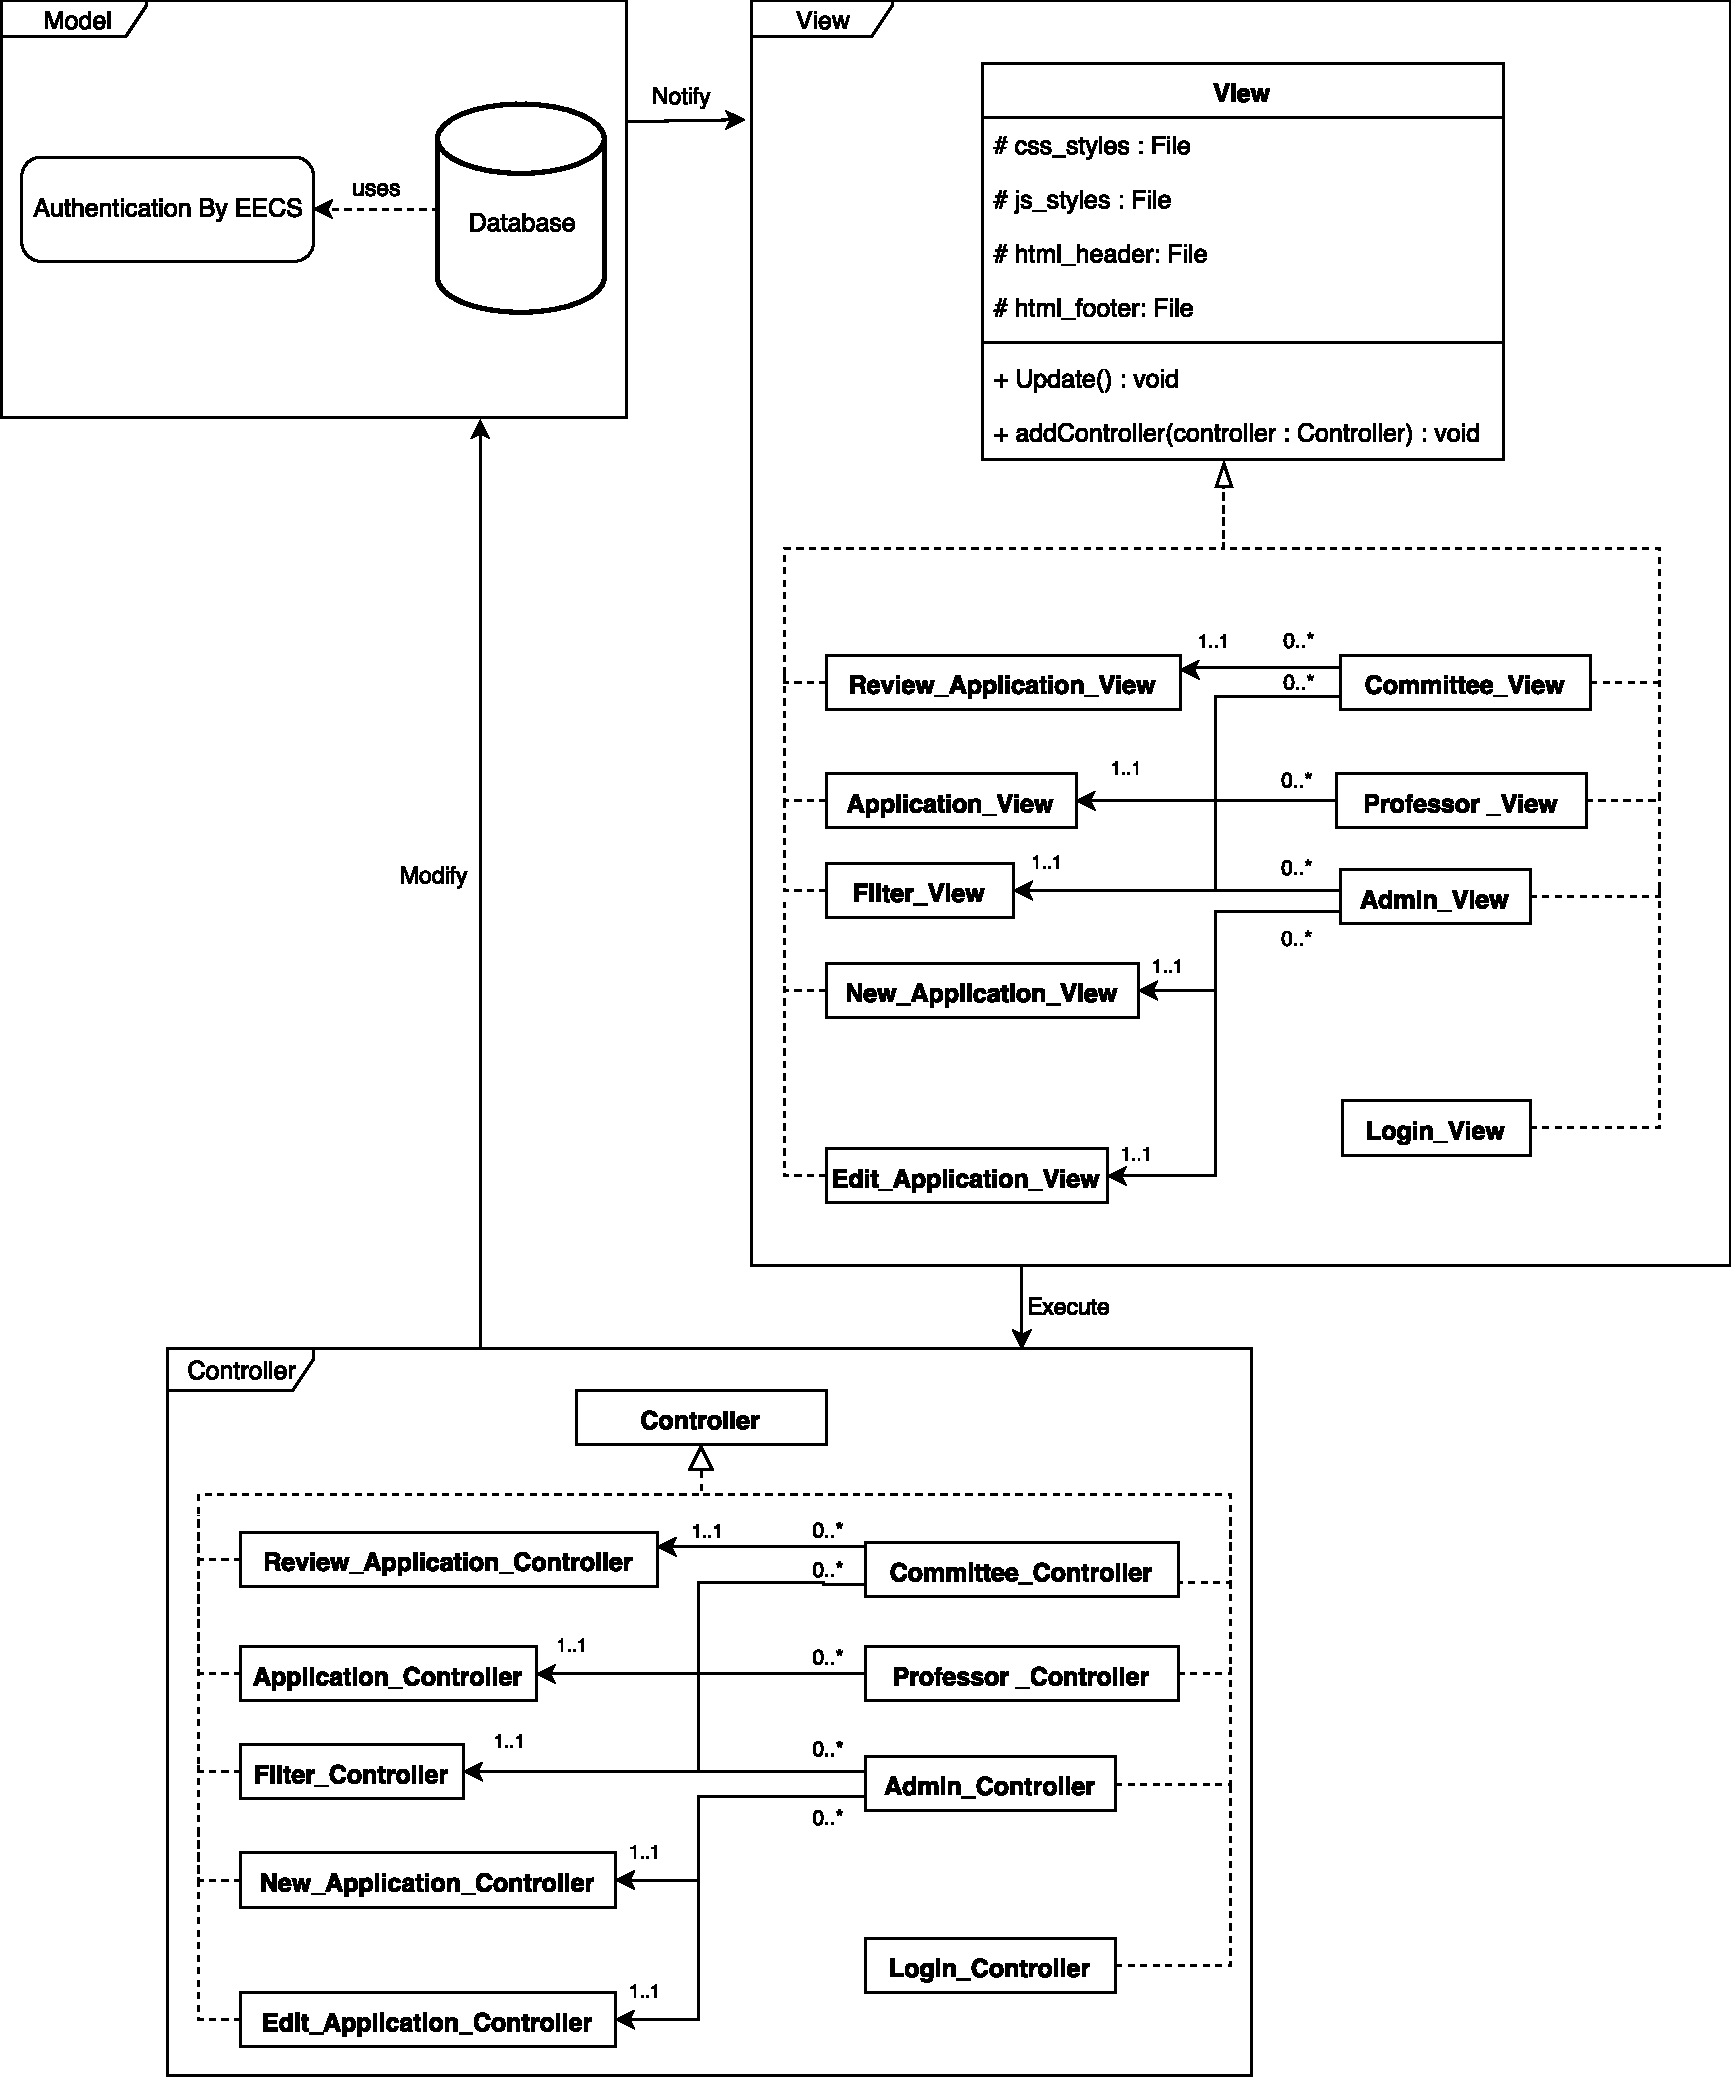
\includegraphics[width=.85\textwidth]{images/class_diagram.pdf}
\end{center}
\caption{UML Class Diagram}
\label{fig:uml_class_diagram}
\end{figure}

\newpage
\subsection{File Structure}
\hl{The next page contains a condensed version of the current file structure of our application. The system is currently run on Node.js and uses the app.js file to start the application. Authentication is done through passport.js. \\ \\ To view all \emph{Controller} related the main folders of focus will be the \emph{routes} and \emph{controller} folder. The routes handles the management of users that traverse to the website and separates what the user can and cannot do based on their role. Each route makes use of the files in the controller  that will directly interact with our model. This is all done on the server. \\
\\ To view all \emph{Model} related files you will need to see the mysql database in addition to the .private folder. the .private folder contains a .htpasswd file of all our users in the system with the files in the model folder to handle the manipulation of the file. \\
\\ Lastly, the \emph{View} related files can be seen in the views folder. All the files contain a html template that will change according to the data received by the model and will provide forms and buttons for the user to communicate with the controller via GET and POST requests. It's stylings can be found in the public folder which contains any client sided javascript, css, images, fonts, and documents.}

\clearpage
\newpage 
\lstinputlisting[caption=File Structure]{images/tree.txt}
\clearpage
\newpage 
\subsection{Decomposition Description}

The System Architecture was designed with the MVC Pattern in mind.

\begin{itemize}
\item The \emph{Model} represents the database and acts as a data handler for all the data to be stored.

\item The \emph{View} represents the front-end web application using web technologies such as html, css and javascript. 

\item The \emph{Controller} represents the back-end system that triggers the model and updates the view.
\end{itemize}


\subsection{Design Rationale}

\subsubsection{MVC}

Given that this is a web application designing it using the MVC pattern makes the most sense here for the following reason:

\begin{itemize}
\item Simultaneous development
\item Ease of modification
\item Multiple Views for our one model
\end{itemize}

As a result of MVC, developers will be able to work on parts of the system concurrently as opposed to having to wait for others to finish their part and the ability to add or remove a feature later on will be easier and the overall system will be modular.

\subsubsection{Roles}

To satisfy the specification requirements of faculty members being able to have more than one role, there is no inheritance/generalization between  faculty members and all the other roles. This design choice allows for an easy separation of information across roles so that changes in one does not affect changes in another.

An alternative to this design would have been to split the roles into their own classes. This choice is not beneficial for our system since all of our roles share common things such as id, name, email etc… and would create a lot of duplication in the system. See Section \ref{sec:data_design} for diagram and data description.

%%%%%%%%%%%%%%%%%%%%%%%%%%%%%%%%%%%%%%%%%%%

\newpage
\begin{figure}[!htb]
\section{Data Design} \label{sec:data_design}
\subsection{Data Description}

The following diagram illustrates the UML Entity Relationship. The design of each entity will be represented in the database during the implementation phase.
\begin{center}
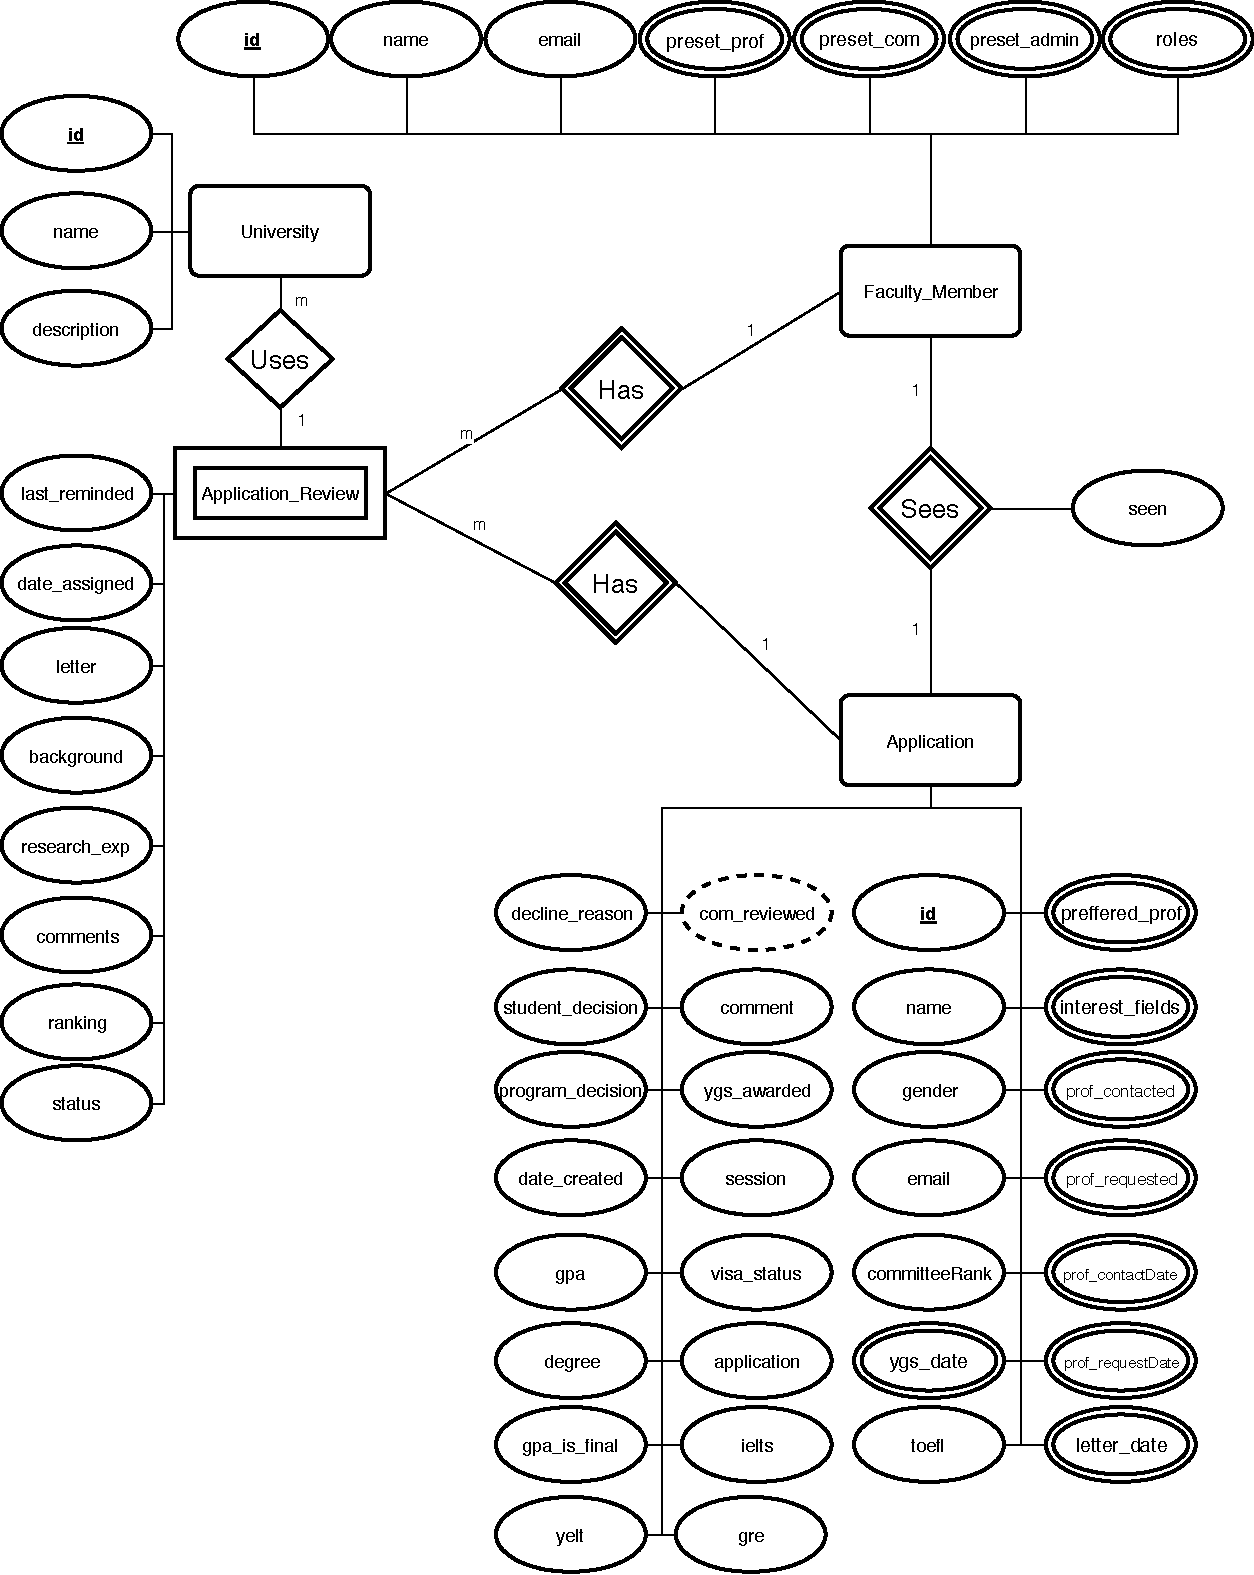
\includegraphics[width=.99\textwidth]{images/entity_relation.pdf}
\end{center}
\caption{Entity Relation Diagram}
\label{fig:uml_entity_diagram}
\end{figure}


\clearpage
\newpage

\begin{figure}[!htb]
\subsection{Data Dictionary}

\begin{center}
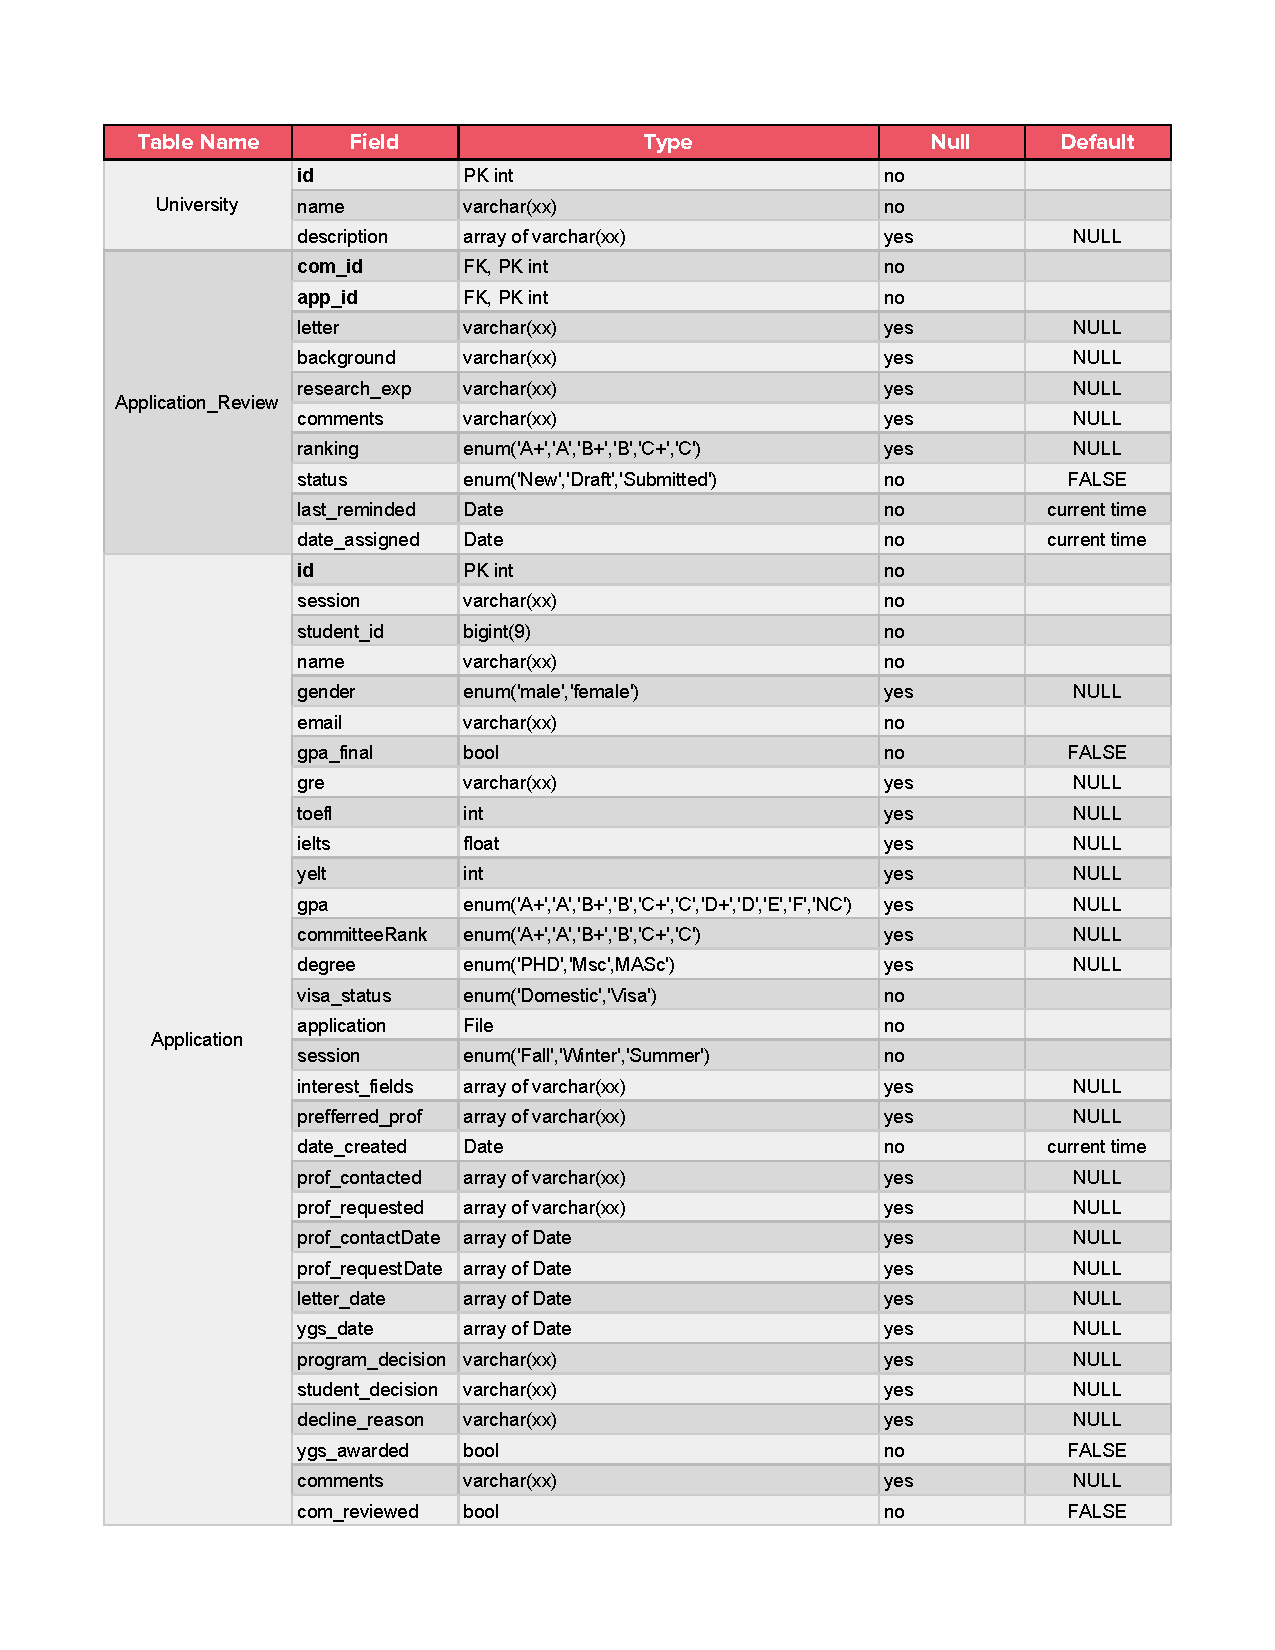
\includegraphics[width=\textwidth, page=1]{images/data_dictionary.pdf}
\end{center}
\caption{\hl{Data Dictionary Part.1}}
\label{fig:dd1}
\end{figure}

\clearpage
\newpage

\begin{figure}[!htb]
\hl{The below figure shows two tables \emph{Fields\_of\_Interest} and \emph{GPA} that are not displayed in our ER-diagram. These two tables are beneficial for the internal logic of our system such as being able to properly sort GPA and to have a more flexibility for things we expect to change throughout the years like fields of interest.}
\begin{center}
\includegraphics[width=\textwidth, page=2]{images/data_dictionary.pdf}
\end{center}
\caption{\hl{Data Dictionary Part.2}}
\label{fig:dd2}
\end{figure}

%%%%%%%%%%%%%%%%%%%%%%%%%%%%%%%%%%%%%%%%%%%

\clearpage
\newpage
\section{Component Design}

\subsection{Model}

The model acts as a data storage handler for the GradApps business system. Most of which is already discussed in Section \ref{sec:data_design}. The database will use MySQL version: 5.7.20 and Authentication By EECS as per the requirements elicited from the client. The design chosen was in favor of simplicity instead of efficiency. This decision was based on the relatively low amount of student applications gradapps will store (roughly 1000 applications per year) thus eliminating the need for faster query calls.

\subsection{View}
Some views will be able to display other views depending on the role selected.

\smallskip 
\noindent Here are a few:

\begin{itemize}
\item Admin View includes the Filter View, New Application View, Edit Application View,  and the Application View.
\item Committee View includes the Filter View, and the Review Application View.
\item Professor View includes the Application View, and the Filter View.
\end{itemize}

\noindent Based on what the main view is (Admin, Committee, Professor) the filter view will adjust accordingly to allow for their respective controllers.


\subsection{Controller}

Since some roles have different privileges than others, it is important to restrict what one user could do based on the view that they are in. For example, if someone is in the professor view they cannot access methods from the admin controller.

\subsubsection{Sequence Diagrams}

The following sequence diagrams describe the communication between our actors and the system under description. In short our system behaves as follows.

\begin{itemize}
\item Actor acts on the system
\item Client side validation
\item Appropriate updates to database
\item Return updated results and error message if necessary.
\end{itemize}

\begin{figure}[!htb]
\begin{center}
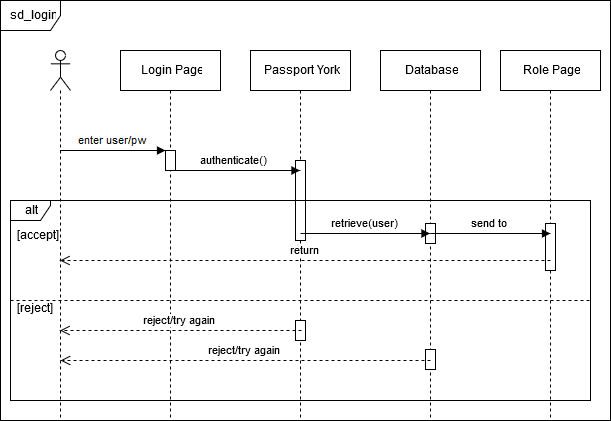
\includegraphics[width=.99\textwidth]{images/sd_login.png}
\end{center}
\caption{Sequence Diagram: Login to the system}
\label{fig:sd_login}
\end{figure}

\begin{figure}[!htb]
\begin{center}
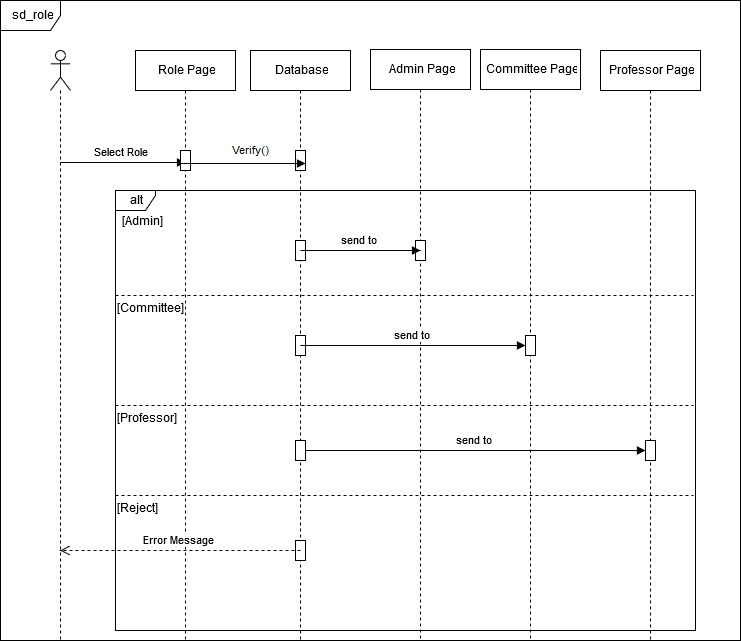
\includegraphics[width=.99\textwidth]{images/sd_role.png}
\end{center}
\caption{Sequence Diagram: Role Selection}
\label{fig:sd_role_selection}
\end{figure}

\begin{figure}[!htb]
\begin{center}
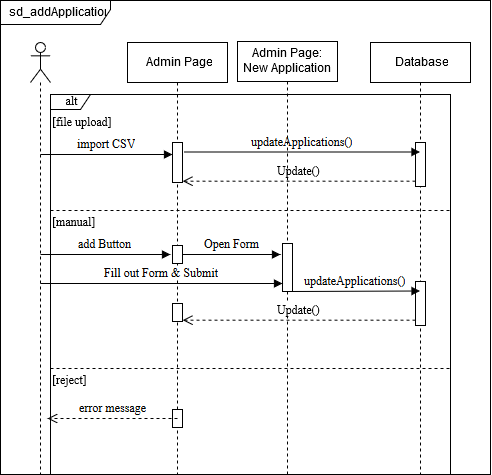
\includegraphics[width=.99\textwidth]{images/sd_addApplication.png}
\end{center}
\caption{Sequence Diagram: Upload an Application}
\label{fig:sd_add_application}
\end{figure}

\begin{figure}[!htb]
\begin{center}
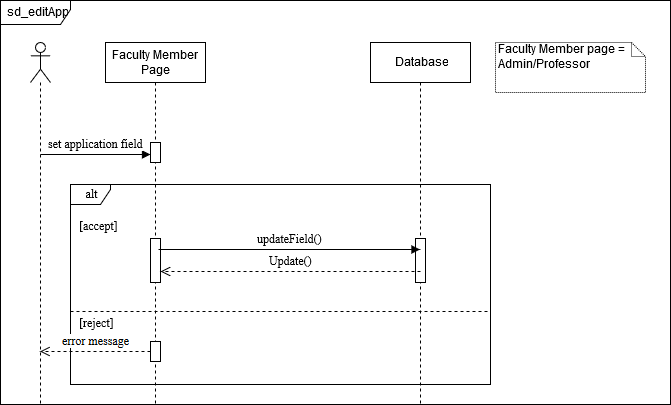
\includegraphics[width=.99\textwidth]{images/sd_editApp.png}
\end{center}
\caption{Sequence Diagram: Update an Application}
\label{fig:sd_update_application}
\end{figure}

\begin{figure}[!htb]
\begin{center}
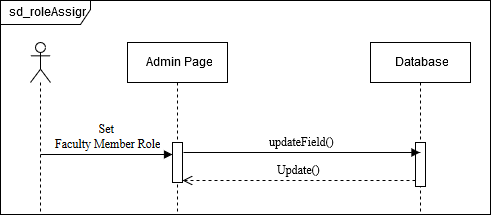
\includegraphics[width=.99\textwidth]{images/sd_roleAssign.png}
\end{center}
\caption{Sequence Diagram: Assigning a Role}
\label{fig:sd_assign_role}
\end{figure}

\begin{figure}[!htb]
\begin{center}
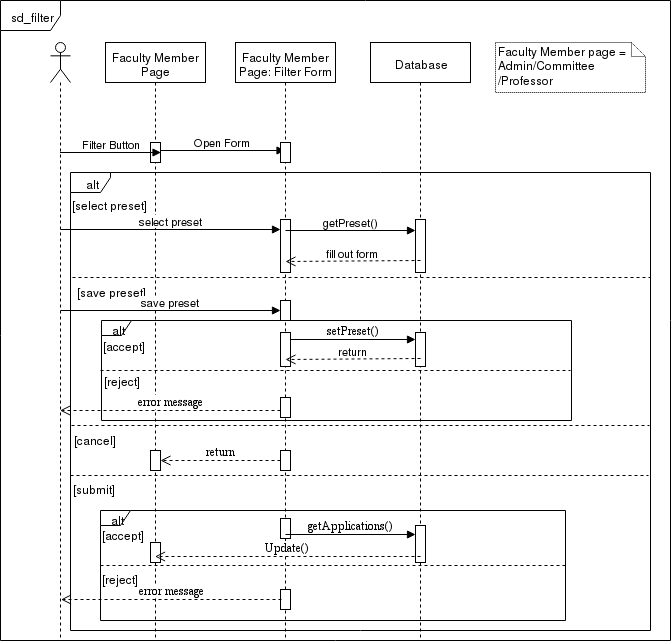
\includegraphics[width=.99\textwidth]{images/sd_filter.png}
\end{center}
\caption{Sequence Diagram: Applying filter}
\label{fig:sd_apply_filter}
\end{figure}

\begin{figure}[!htb]
\begin{center}
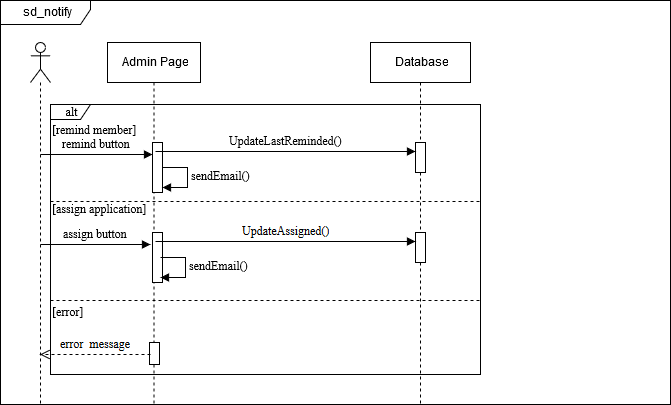
\includegraphics[width=.99\textwidth]{images/sd_notify.png}
\end{center}
\caption{Sequence Diagram: Notification}
\label{fig:sd_notification}
\end{figure}

\begin{figure}[!htb]
\begin{center}
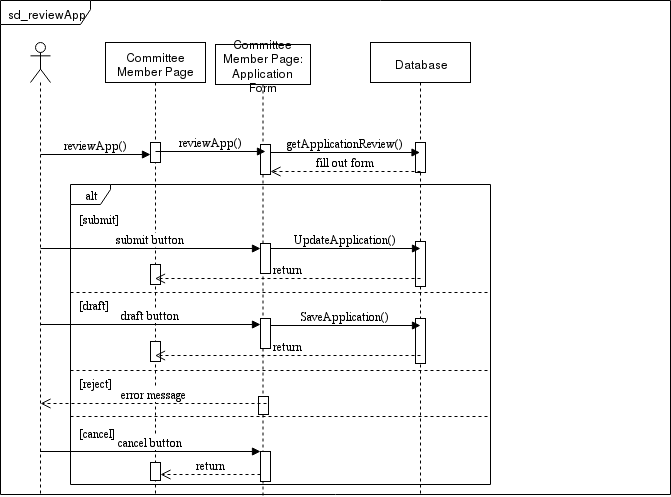
\includegraphics[width=.99\textwidth]{images/sd_reviewApp.png}
\end{center}
\caption{Sequence Diagram: Review an Application}
\label{fig:sd_review_application}
\end{figure}

\begin{figure}[!htb]
\begin{center}
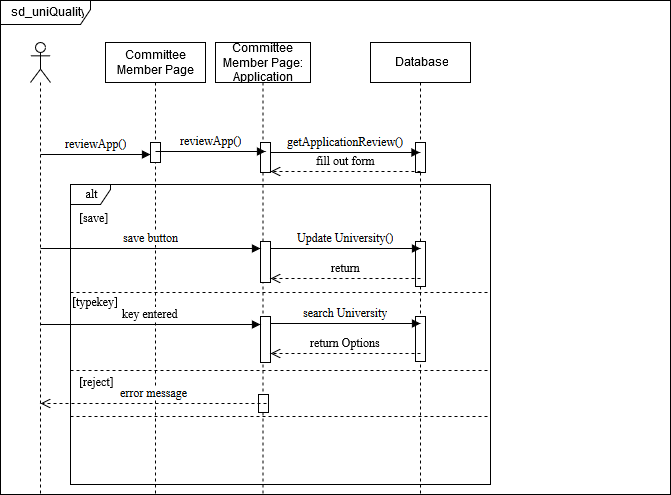
\includegraphics[width=.99\textwidth]{images/sd_uniQuality.png}
\end{center}
\caption{Sequence Diagram: Applying University Assessment}
\label{fig:sd_apply_uni}
\end{figure}


%%%%%%%%%%%%%%%%%%%%%%%%%%%%%%%%%%%%%%%%%%%

\clearpage
\newpage
\section{Human Interface Design}

\subsection{Overview of User Interface}

Refer to \url{http://cambridge.eecs.yorku.ca:3000/}

\subsection{Screen Images}

\begin{figure}[!htb]
\begin{center}
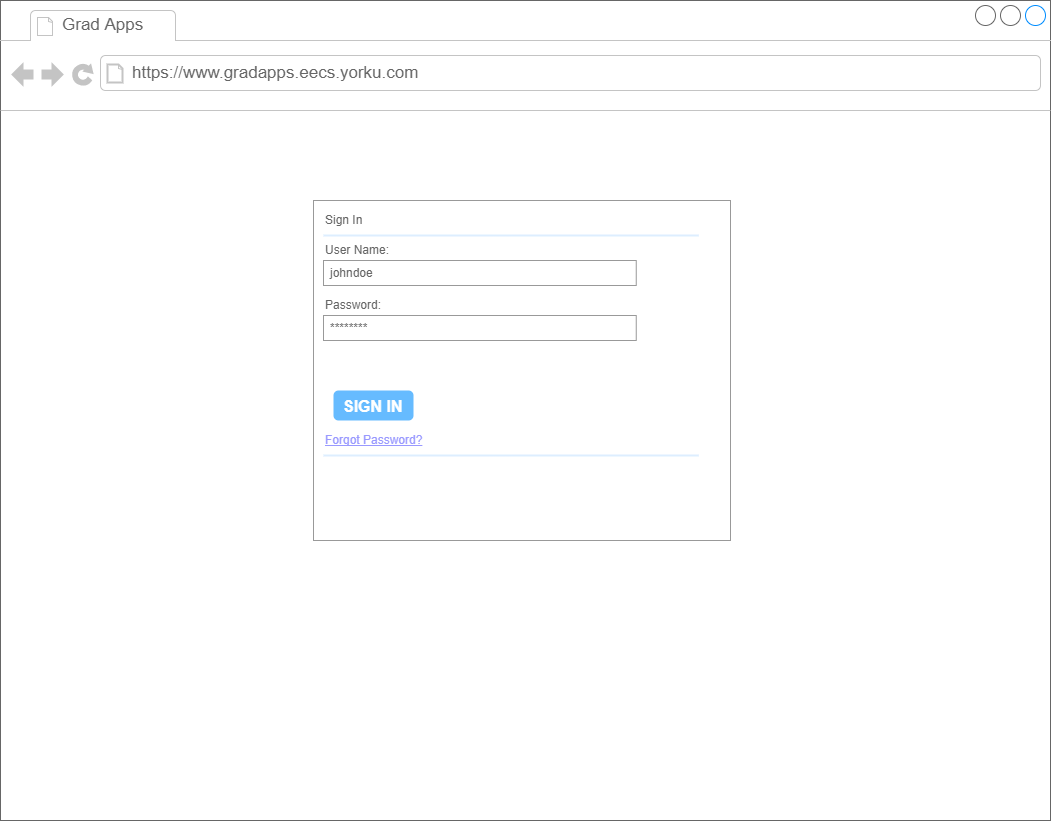
\includegraphics[width=.99\textwidth]{images/login_page.png}
\end{center}
\caption{Login Page View}
\label{fig:login_page_view}
\end{figure}

\begin{figure}[!htb]
\begin{center}
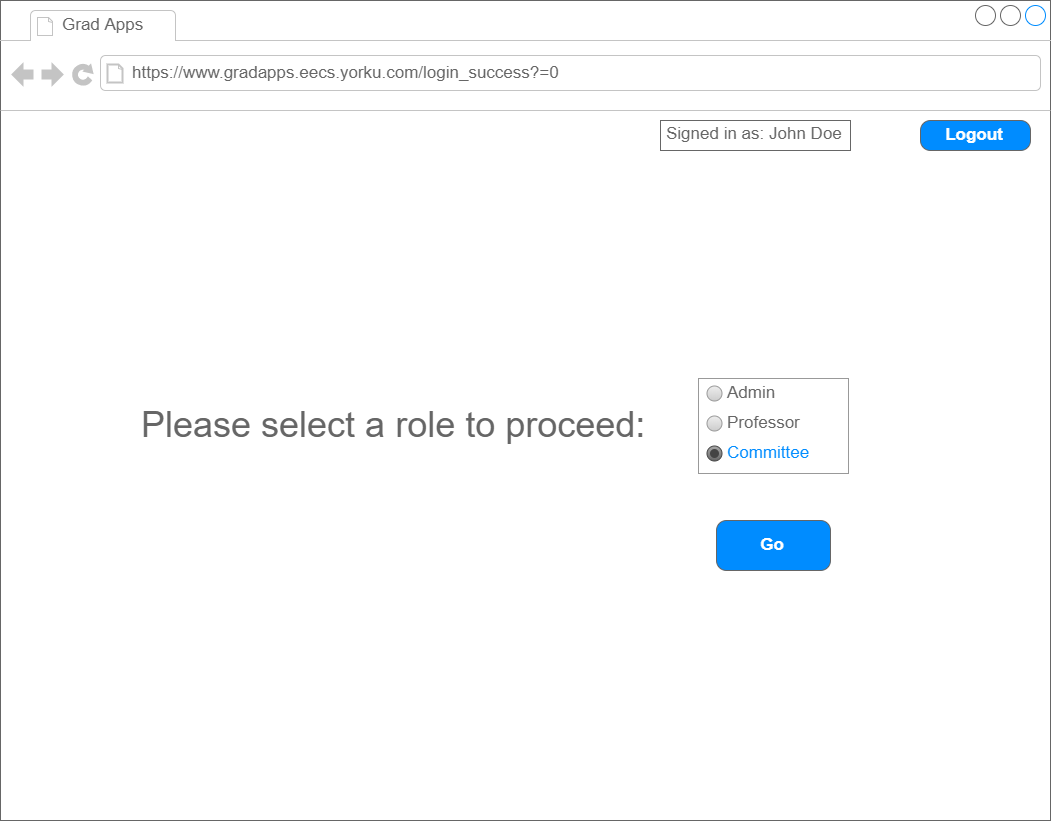
\includegraphics[width=.99\textwidth]{images/role_selection.png}
\end{center}
\caption{Role Selection View}
\label{fig:role_selection_view}
\end{figure}

\begin{figure}[!htb]
\begin{center}
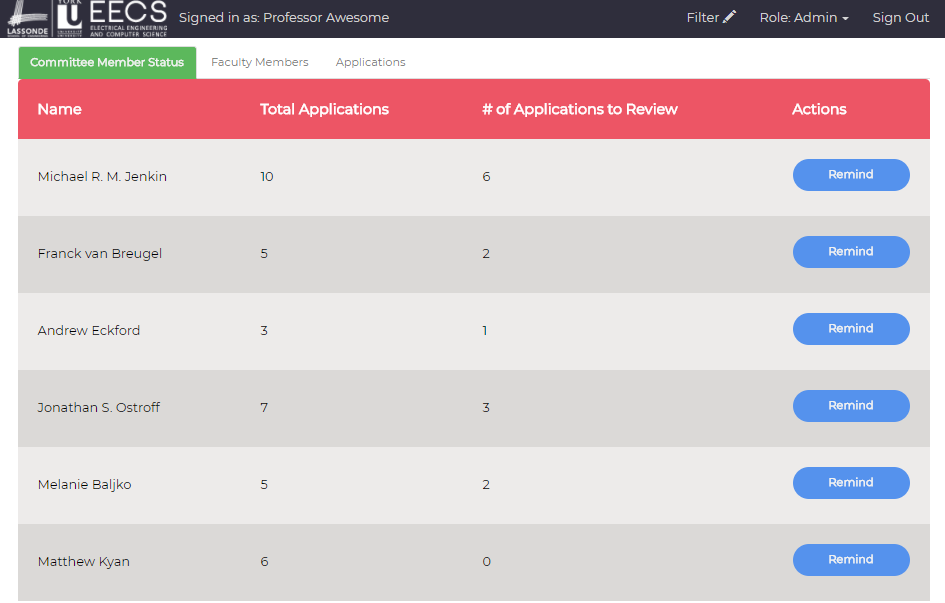
\includegraphics[width=.78\textwidth]{images/admin_view1.png}
\end{center}
\caption{Admin View - Committee Member Status}
\label{fig:admin_view1}
\end{figure}

\begin{figure}[!htb]
\begin{center}
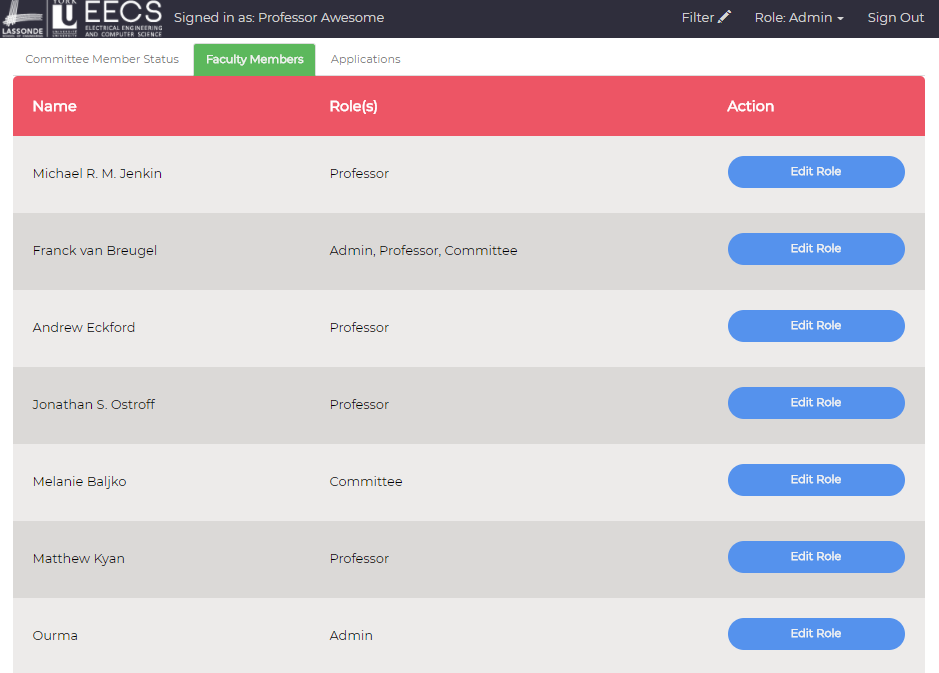
\includegraphics[width=.78\textwidth]{images/admin_view2.png}
\end{center}
\caption{Admin View - List Faculty Members}
\label{fig:admin_view2}
\end{figure}

\begin{figure}[!htb]
\begin{center}
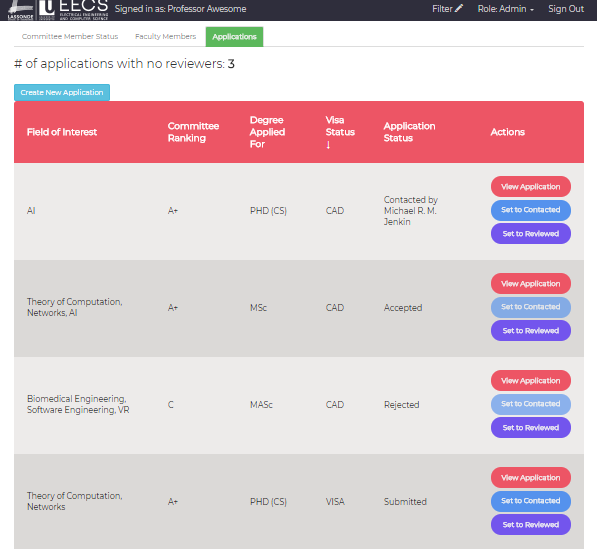
\includegraphics[width=.99\textwidth]{images/admin_prof_view.png}
\end{center}
\caption{Admin and Professor View - List of Student Applications}
\label{fig:admin_prof_view}
\end{figure}

\begin{figure}[!htb]
\begin{center}
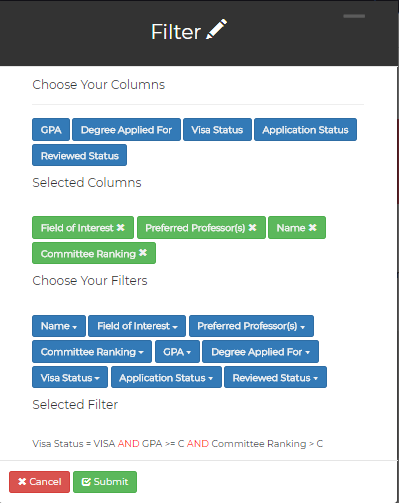
\includegraphics[width=.78\textwidth]{images/admin_prof_filter.png}
\end{center}
\caption{Filters available for the Admin and Professor role}
\label{fig:admin_prof_filter}
\end{figure}

\begin{figure}[!htb]
\begin{center}
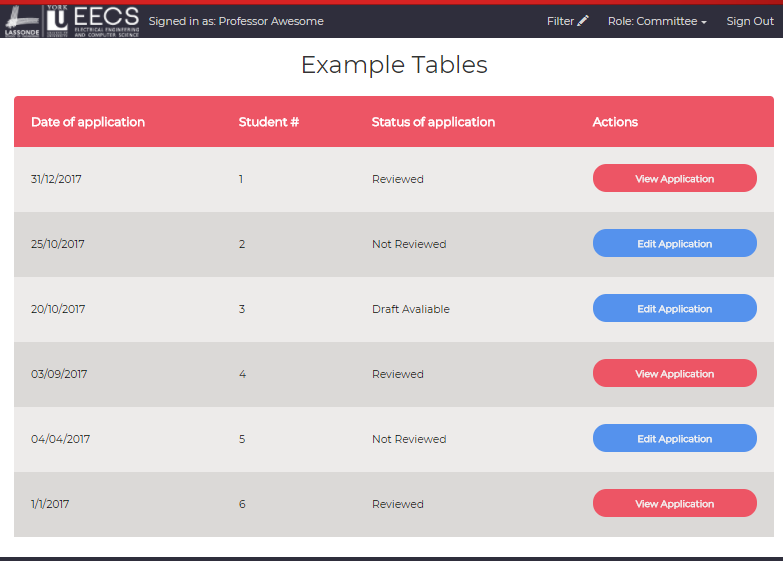
\includegraphics[width=.99\textwidth]{images/committee_view.png}
\end{center}
\caption{Committee View - List of review applications}
\label{fig:committee_view}
\end{figure}

\begin{figure}[!htb]
\begin{center}
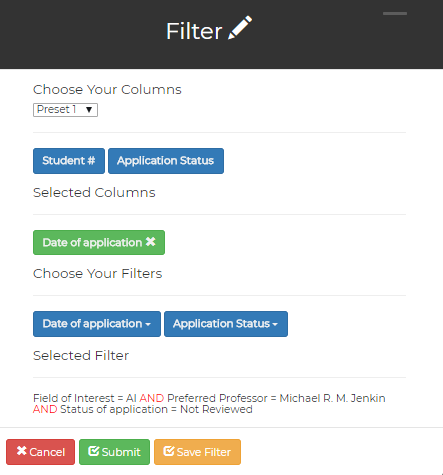
\includegraphics[width=.78\textwidth]{images/committee_filter.png}
\end{center}
\caption{Filters available for the Committee role}
\label{fig:committee_filter}
\end{figure}

\clearpage
\newpage
\subsection{Screen Objects and Actions}

The screenshots un the previous section from Figure \ref{fig:login_page_view} to \ref{fig:committee_filter} describes the flow of action an user may take for the System Under Description. The following describes each figure from the previous section.

\begin{itemize}
\item Figure \ref{fig:login_page_view} specifies the login view for the system. The login credentials shall be authenticated by Passport York. The user is expected to have a valid Passport York account and be part of the system database in order to gain access to the system.
\item Figure \ref{fig:role_selection_view} specifies the role selection view upon logging into the system. Once the user has been successfully authenticated into the system, the user needs to select a role to proceed further.
\item Figure \ref{fig:admin_view1} specifies the admin view of checking the committee member status. This view includes reminding a committee member who have been assigned a review and has not completed it yet.
\item Figure \ref{fig:admin_view2} specifies the admin view that lists all the members in the system. An admin can remove or change a role of a member. An admin can further add a new member into the system.
\item Figure \ref{fig:admin_prof_view} specifies the admin and professor view of all student applications in the system.
\item Figure \ref{fig:admin_prof_filter} specifies the admin and professor view of the filters available on student applications.
\item Figure \ref{fig:committee_view} specifies the committee member view of all applications needed for review in the system.
\item Figure \ref{fig:committee_filter} specifies the committee member view of the filters available on review applications.
\end{itemize}

%%%%%%%%%%%%%%%%%%%%%%%%%%%%%%%%%%%%%%%%%%%

\end{document}  
